\documentclass[tikz, border=5, convert]{standalone}

\begin{document}

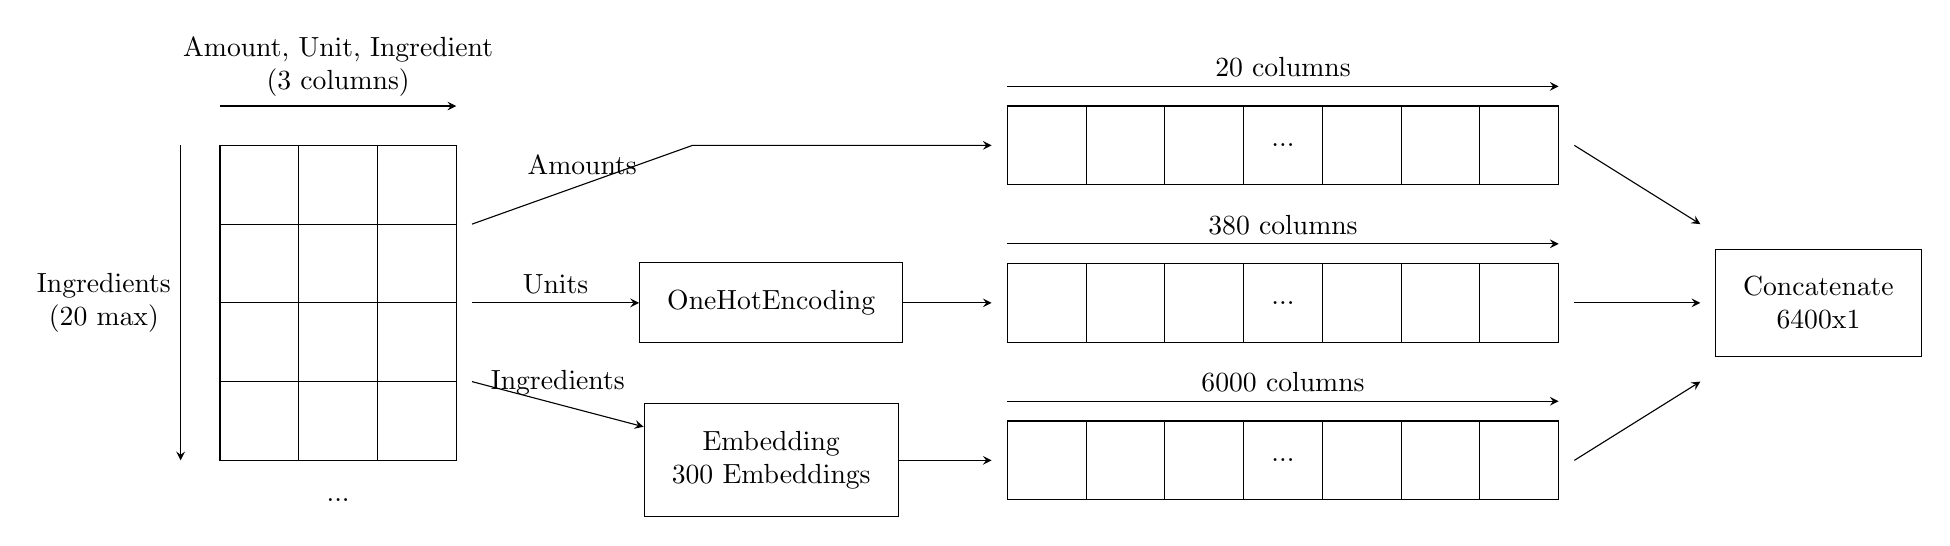
\begin{tikzpicture}[>=stealth]


\foreach \x in {0,...,2}
  	\foreach \y in {0,...,3}
    	\filldraw [fill=white] (\x, \y) -- (\x+1, \y) -- (\x+1, \y+1) --
      			(\x, \y+1) -- cycle (\x+.5, \y+.5) node [yslant=tan(15)] {};
\draw [->] (0, 4.5)  -- (3, 4.5)   node [midway, above, align=center] {Amount, Unit, Ingredient\\(3 columns)};
\draw [->] (-.5, 4)  -- (-.5, 0)   node [midway, left, align=center] {Ingredients\\(20 max)};
\draw (1.5,-0.5) node {...}; 


\node [draw=black, inner sep=10pt] (oneHot) at (7,2) {OneHotEncoding};
\node [draw=black, inner sep=10pt, align=center] (embedding) at (7,0) {Embedding\\300 Embeddings};

\draw [->] (3.2,3) -- (6,4) node [midway, above, align=center] {Amounts} -- (9.8,4);
\draw [->] (3.2,2) -- (oneHot) node [midway, above, align=center] {Units};
\draw [->] (3.2,1) -- (embedding) node [midway, above, align=center] {Ingredients};

\draw [->] (oneHot) -- (9.8,2);
\draw [->] (embedding) -- (9.8,0);


\foreach \x in {10,...,16}
  	\foreach \y in {3.5,...,3.5}
    	\filldraw [fill=white] (\x, \y) -- (\x+1, \y) -- (\x+1, \y+1) --
      			(\x, \y+1) -- cycle (\x+.5, \y+.5) node [yslant=tan(15)] {};
\draw (13.5,4) node {...}; 
\draw [->] (10,4.75) -- (17,4.75) node[midway, above, align=center] {20 columns};

\foreach \x in {10,...,16}
  	\foreach \y in {1.5,...,1.5}
    	\filldraw [fill=white] (\x, \y) -- (\x+1, \y) -- (\x+1, \y+1) --
      			(\x, \y+1) -- cycle (\x+.5, \y+.5) node [yslant=tan(15)] {};
\draw (13.5,2) node {...}; 
\draw [->] (10,2.75) -- (17,2.75) node[midway, above, align=center] {380 columns};

\foreach \x in {10,...,16}
  	\foreach \y in {-0.5,...,-0.5}
    	\filldraw [fill=white] (\x, \y) -- (\x+1, \y) -- (\x+1, \y+1) --
      			(\x, \y+1) -- cycle (\x+.5, \y+.5) node [yslant=tan(15)] {};
\draw (13.5,0) node {...}; 
\draw [->] (10,0.75) -- (17,0.75) node[midway, above, align=center] {6000 columns};

\draw [->] (17.2, 4) -- (18.8, 3);
\draw [->] (17.2, 2) -- (18.8, 2);
\draw [->] (17.2, 0) -- (18.8, 1);

\node [draw=black, inner sep=10pt, align=center] (concat) at (20.3,2) {Concatenate\\6400x1};
	
\end{tikzpicture}
	
\end{document}
